\vspace{-0.3cm}
\section{Methodology}
\label{sec:method}
\vspace{-0.2cm}


\begin{figure}[!t]
    \centering
    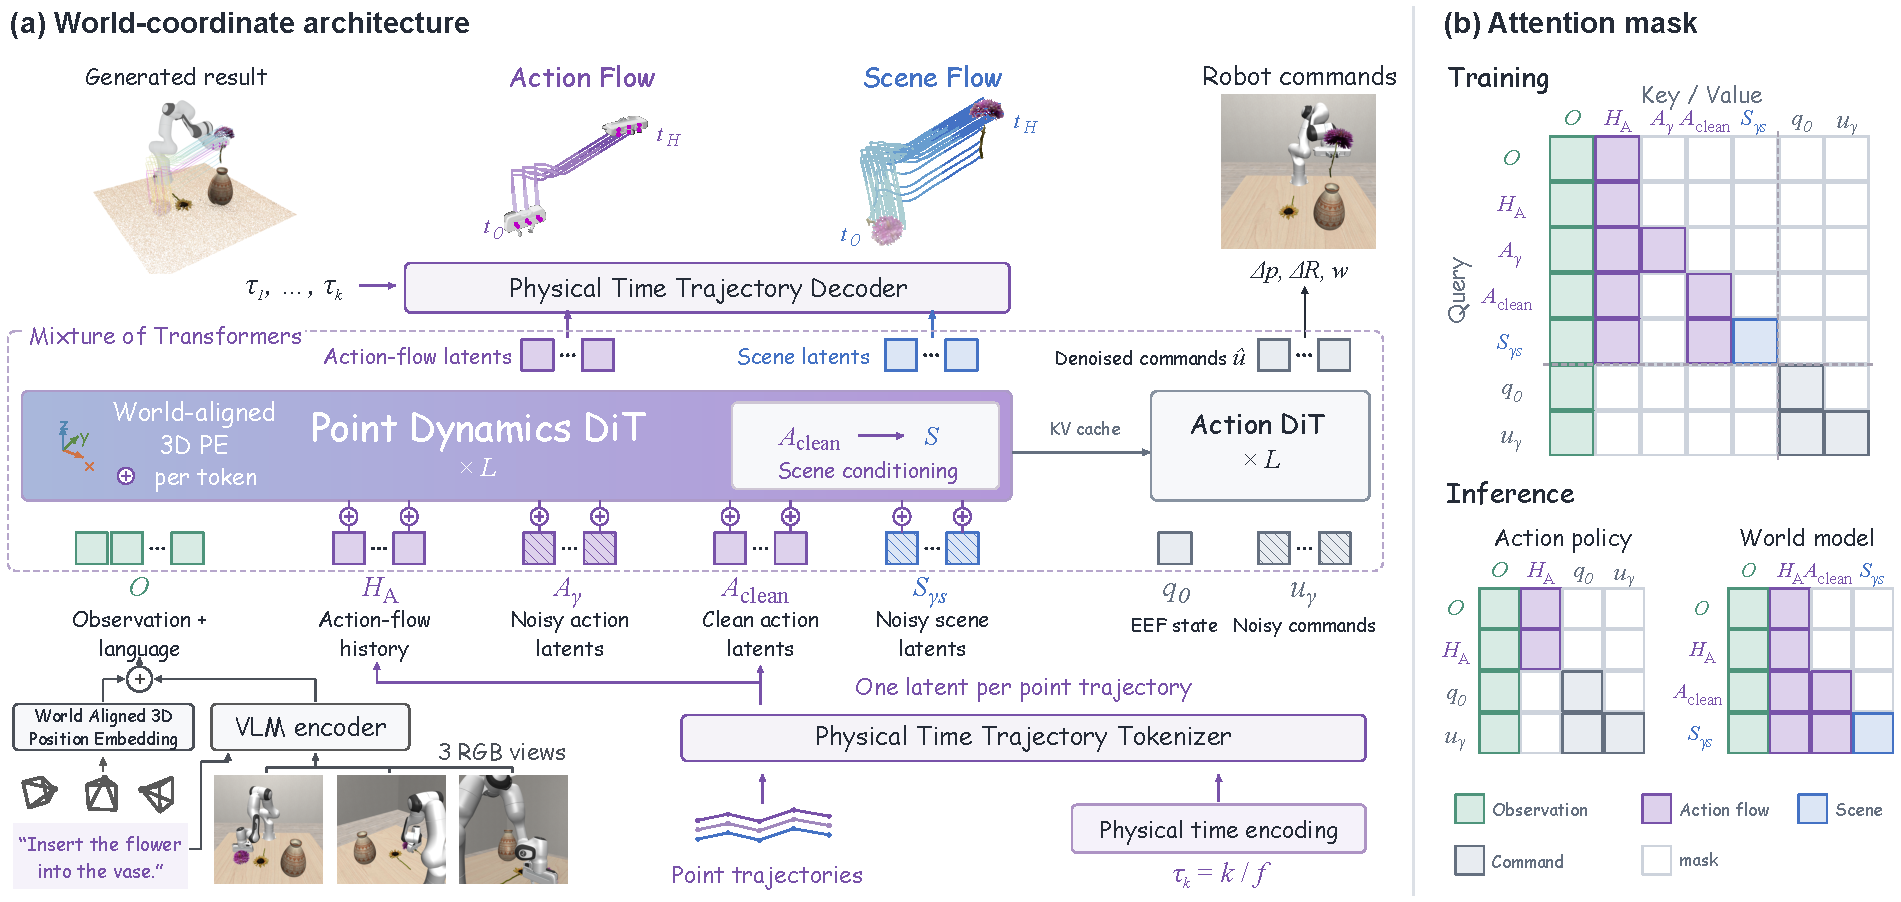
\includegraphics[width=\linewidth]{figures/architecture.pdf}
    \vspace{-0.7cm}
    \caption{\textbf{\method{} architecture and attention masks.}
    Left: The point dynamics expert models both action and scene flows, while the action
    expert generates the end-effector action chunk. Scene flow generation is conditioned
    on clean demonstrated action flow during training and generated or supplied action flow at inference.
    Right: Colored/white cells indicate
    allowed/blocked attention. Policy-only inference omits both future action-flow and scene-flow tokens.}
    \vspace{-0.3cm}
    \label{fig:architecture}
    \label{fig:attention_mask}
\end{figure}

We first revisit video-based world action modeling, then formulate
\method{} in a shared metric 3D frame, as illustrated in
Fig.~\ref{fig:architecture}.

\vspace{-0.2cm}
\subsection{Revisiting Video World Action Models}
\label{sec:method:video_wam}
\vspace{-0.2cm}

Let $o$ denote current image observations, $\ell$ the instruction,
$a_{1:H}$ an action chunk, and $v_{1:T}$ future images.
Video-based WAMs represent future interactions through images or visual
latents. For models that condition actions on predicted futures, the
action distribution can be written as
\begin{equation}
    p(a_{1:H}\mid o,\ell)
    =\int p(v_{1:T}\mid o,\ell)\,
    p(a_{1:H}\mid o,\ell,v_{1:T})\,dv_{1:T}.
    \label{eq:video_wam}
\end{equation}
Future videos and actions may be generated jointly or sequentially.
Fast-WAM~\citep{yuan2026fastwam} instead retains video co-training but
omits future-video generation at inference:
\begin{equation}
    p_{\theta}(a_{1:H}\mid o,\ell)
    =p_{\theta}\!\left(a_{1:H}\mid z(o,\ell)\right),
    \qquad
    \mathcal L
    =\mathcal L_{\mathrm{act}}+\lambda\mathcal L_{\mathrm{vid}}.
    \label{eq:fastwam}
\end{equation}
Its video backbone encodes the current observation and instruction into
$z(o,\ell)$ in one forward pass, while the action expert still performs
iterative denoising. This removes future-video sampling, but the shared
representation remains image-based, without an explicit metric 3D frame.

\vspace{-0.2cm}
\subsection{3D-Native World Action Formulation}
\label{sec:method:formulation}
\vspace{-0.2cm}

At time $t$, context $\mathcal C$ comprises the instruction $\ell$,
multi-view observations $\mathcal O_t=\{\mathcal O_{t,i}\}_{i=1}^{N_v}$,
camera calibration $\{\mathbf K_i,\mathbf T^W_{t,i}\}_{i=1}^{N_v}$,
and historical action flow $\mathcal H_{\mathrm A}$.
Here $\mathbf K_i$ denotes camera intrinsics, and
$\mathbf T^W_{t,i}\in\mathrm{SE}(3)$ maps camera coordinates into the
metric frame $\mathcal F^W$, fixed within each prediction window.
Action prediction additionally uses the current end-effector state
$\mathbf q_0$.

Given query points and future timestamps, we predict action flow
$\mathbf A$ for the interacting body and scene flow $\mathbf S$ for
the environment, both as displacement trajectories in $\mathcal F^W$.
A separate action branch predicts an executable end-effector action
chunk $\mathbf u$. Our model factorizes their joint distribution as
\begin{equation}
    p_{\theta}(\mathbf A,\mathbf u,\mathbf S\mid\mathcal C,\mathbf q_0)
    =
    p_{\theta}(\mathbf A\mid\mathcal C)\,
    p_{\theta}(\mathbf u\mid\mathcal C,\mathbf q_0)\,
    p_{\theta}(\mathbf S\mid\mathbf A,\mathcal C).
    \label{eq:physwam_factorization}
\end{equation}
Action flow and the action chunk can be sampled in parallel; scene prediction
then conditions on generated action flow $\widehat{\mathbf A}$ or an
externally supplied trajectory $\mathbf A_{\mathrm{ext}}$ in simulator
mode. Policy-only execution evaluates only
$p_{\theta}(\mathbf u\mid\mathcal C,\mathbf q_0)$, omitting both point flows.
The following sections describe spatial grounding, the shared trajectory
representation, and the coupled experts that implement these factors.

\vspace{-0.2cm}

\subsection{World-Aligned Observations}
\label{sec:method:observation}
\vspace{-0.2cm}

\noindent\textbf{Frame alignment.}
Within each prediction window, observations, robot or human motion, and
scene trajectories share one fixed metric frame.
Robot demonstrations use a robot-base or shared embodiment frame.
Egocentric human demonstrations use the camera frame of the window anchor,
held fixed throughout the window.
Appendix~\ref{app:dataset_visualization} lists the dataset conventions.

\noindent\textbf{World-aligned 3D position embedding.}
Each visual token receives a position embedding in the world frame.
For a view with valid depth,
$\mathcal O_{t,i}=(\mathbf I_{t,i},\mathbf D_{t,i})$ contains the RGB
image and the depth along the optical axis.
The vision encoder maps the image to a token grid
$\mathbf F_{t,i}=\operatorname{Enc}_{\mathrm{vis}}(\mathbf I_{t,i})$.
We back-project each pixel and transform it into world coordinates,
\begin{equation}
    \mathbf P_{\mathrm{camera},i}(u,v)
    =\mathbf D_{t,i}(u,v)\,\mathbf K_i^{-1}[u,v,1]^\top,
    \qquad
    \begin{bmatrix}
        \mathbf P_{\mathrm{world},i}(u,v)\\ 1
    \end{bmatrix}
    =\mathbf T^W_{t,i}
    \begin{bmatrix}
        \mathbf P_{\mathrm{camera},i}(u,v)\\ 1
    \end{bmatrix}.
    \label{eq:world_coordinate_map}
\end{equation}
Here, $(u,v)$ denotes pixel-center coordinates, and the time index is
omitted from the coordinate maps.
A fixed Fourier map $\boldsymbol\psi$ encodes the world position.
Inside each patch, $\operatorname{Enc}_{\mathrm{3D}}$ applies
$\boldsymbol\psi$ and projects the result to the visual-token dimension:
\begin{equation}
    \mathbf E_{\mathrm{pos},t,i}
    =\operatorname{Enc}_{\mathrm{3D}}(\mathbf P_{\mathrm{world},i}),
    \qquad
    \widetilde{\mathbf F}_{t,i}
    =\mathbf F_{t,i}+\mathbf E_{\mathrm{pos},t,i}.
    \label{eq:depth_position_embedding}
\end{equation}

\noindent\textbf{Spatial grounding without observed depth.}
Without depth, the position embedding is computed from a weighted
combination of positional features along the camera ray.
For a patch centered at $(u,v)$, we draw $M=64$ depths uniformly from
$0.1$ to $2.0\,\mathrm{m}$, back-project them by
Eq.~\ref{eq:world_coordinate_map}, and score them with the patch feature
$\mathbf f$:
\begin{equation}
\begin{aligned}
    \alpha_m
    &=\operatorname{softmax}_{m}
    \left(
        \frac{(\mathbf W_q\mathbf f)^\top
        \mathbf W_k\boldsymbol\psi(\mathbf p_{\mathrm{camera},m})}
        {\sqrt{d}}
    \right),\\
    \mathbf E_{\mathrm{ground}}
    &=\mathbf W_o\sum_{m=1}^{M}
        \alpha_m\mathbf W_v
        \boldsymbol\psi(\mathbf p_{\mathrm{world},m}).
\end{aligned}
\label{eq:frustum_routing}
\end{equation}
Here $\mathbf f\in\mathbb R^{d_f}$ is the patch feature and
$\boldsymbol\psi(\cdot)\in\mathbb R^{d_\psi}$, with
$\mathbf W_q\in\mathbb R^{d\times d_f}$,
$\mathbf W_k\in\mathbb R^{d\times d_\psi}$, and
$\mathbf W_v\in\mathbb R^{d\times d_\psi}$.
Keys encode camera-frame positions, and values encode the same candidates
in the world frame.
$\mathbf E_{\mathrm{ground}}$ is added to the visual tokens in place of
$\mathbf E_{\mathrm{pos},t,i}$ in Eq.~\ref{eq:depth_position_embedding}.
Where depth is reliable, we use depth-derived embeddings and supervise
the routing weights by matching Fourier features:
\begin{equation}
    \mathcal L_{\mathrm{PE}}
    =\sum_{i=1}^{N_v}
    \mathbb E_{\mathcal R\in\mathcal V_i}
    \left\|
        \sum_{m=1}^{M}\alpha_m
        \boldsymbol\psi(\mathbf p_{\mathrm{world},m})
        -\operatorname{sg}\!\left(
            \operatorname{Avg}_{(u,v)\in\mathcal R}
            \boldsymbol\psi(\mathbf P_{\mathrm{world},i}(u,v))
        \right)
    \right\|_2^2 .
    \label{eq:position_distillation}
\end{equation}
Here $\mathcal V_i$ contains regions with reliable depth in view $i$,
and $\operatorname{sg}$ denotes stop-gradient. Only valid-depth pixels
contribute to the target average.
With this module, \method{} pretrains jointly on RGB and RGB-D data, and depth may be absent at inference.
Appendix~\ref{app:missing_depth} evaluates the router when depth is
removed at test time.

\vspace{-0.2cm}
\subsection{Physical-Time Point-Flow Representation}
\label{sec:method:flow_representation}
\vspace{-0.2cm}

\noindent\textbf{Action flow and scene flow.}
In the same world frame, action and scene flows describe displacement
from each query point's current position.
For query $n$ at $\mathbf x_{t,n}$, the target is
$\{\Delta\mathbf x_{n,k}\}_{k=1}^{H}$, with
$\Delta\mathbf x_{n,k}=\mathbf x_{t+\tau_k,n}-\mathbf x_{t,n}$.
The elapsed time is $\tau_k$, and point identity is preserved throughout
the trajectory.

For robots, we sample $N_g=20$ points from the URDF-defined gripper
geometry of each arm and retain their link-local coordinates.
Forward kinematics maps these points into the world frame at each
recorded joint configuration, preserving correspondence through arm and
finger motion.
Human demonstrations use 21 MANO-derived keypoints~\citep{romero2017mano}
per observed hand. Following PointWorld~\citep{huang2026pointworld},
we mask robot pixels using the URDF and current joint state, back-project
the remaining RGB-D pixels, and sample $N_s$ scene query points. Simulator states supply ground-truth correspondences
where available and scene-flow loss is applied only to valid trajectories.
At inference, scene prediction requires current 3D query coordinates
from depth or supplied geometry.

\noindent\textbf{Physical-time trajectory tokenizer.}
To better align different trajectories within diverse datasets, we encode time in seconds rather than frame indices, using $\tau_k=k/f$
at sampling rate $f$.
A fixed basis $\boldsymbol\phi_{\mathrm{time}}$ of $\tau/T_{\max}$, with
$T_{\max}=3\,\mathrm{s}$ shared across datasets, gives equal elapsed times
the same features; history uses negative offsets.
An input MLP maps each displacement to $\mathbf h_{n,k}$, and temporal
MLPs map $\boldsymbol\phi_{\mathrm{time}}(\tau_k)$ to FiLM parameters
$(\mathbf a_k,\mathbf b_k)$ for the encoder and the decoder.
The encoder pools the trajectory into one latent, and the decoder reads
that latent back at a requested time:
\begin{equation}
\begin{aligned}
    \mathbf z_n
    &=\frac{1}{\sqrt H}\sum_{k=1}^{H}
    \left[(\mathbf 1+\mathbf a^{\mathrm{enc}}_k)\odot
    \mathbf h_{n,k}+\mathbf b^{\mathrm{enc}}_k\right],\\
    \widehat{\Delta\mathbf x}_{n,k}
    &=\operatorname{MLP}_{\mathrm{out}}
    \left[(\mathbf 1+\mathbf a^{\mathrm{dec}}_k)\odot
    \mathbf z_n+\mathbf b^{\mathrm{dec}}_k\right].
\end{aligned}
\label{eq:physical_time_flowchunk}
\end{equation}
Padding is excluded from the sum.
Action flow, scene flow, and history share this tokenizer, so each point
is one token regardless of trajectory length or sampling density.
Flow tokens are anchored only at current world-frame points:
positional embeddings as in Eq.~\ref{eq:depth_position_embedding}
are added throughout denoising. Decoding gives
$\widehat{\mathbf x}_{t+\tau_k,n}
=\mathbf x_{t,n}+\widehat{\Delta\mathbf x}_{n,k}$.
Appendix~\ref{app:trajectory_tokenizer} gives the basis and the
reconstruction stage.

\begin{figure}[!t]
    \centering
    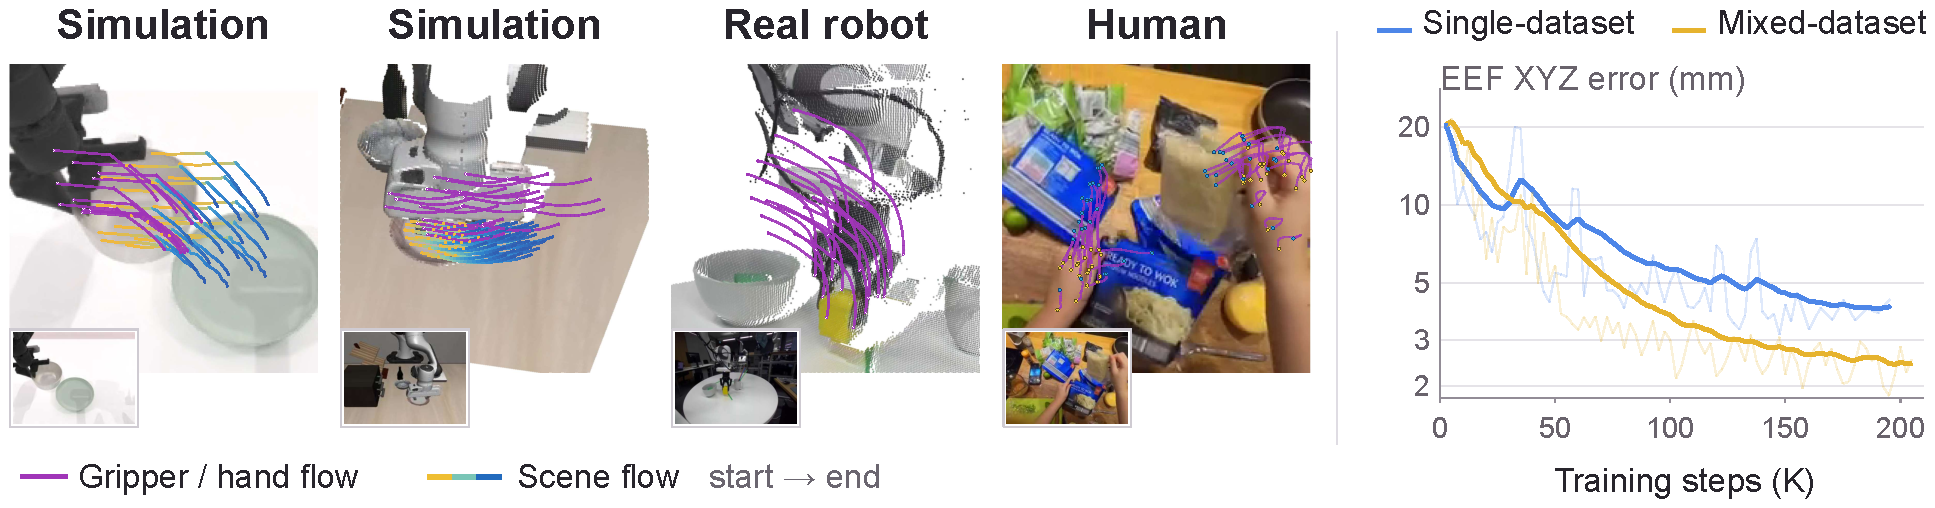
\includegraphics[width=\linewidth]{figures/mixed_dataset_training.pdf}
    \vspace{-0.8cm}
    \caption{\textbf{Shared point-flow representations across data sources.}
    Left: gripper/hand trajectories (purple) and scene trajectories
    (yellow--blue), with RGB insets. Right: RoboTwin end-effector XYZ
    error (mm). Thick curves show exponential moving averages (EMA)
    of the thin curves. \vspace{-0.2cm}}
    \label{fig:experiments:mixed_dataset_training}
\end{figure}

\vspace{-0.2cm}

\subsection{Model Architecture}
\label{sec:method:architecture}
\vspace{-0.2cm}


\noindent\textbf{Coupled experts.}
\method{} uses a Mixture-of-Transformers~\citep{liang2024mixture}
with two diffusion transformers~\citep{peebles2023scalable}:
a point dynamics expert for action and scene flows, and an action expert for the
end-effector action chunk $\mathbf u$. The point dynamics expert processes spatially grounded
primary-view VLM tokens, auxiliary-view features from the shared vision
tower, and historical and future flow latents. At each layer, the smaller
action expert reads the dynamics expert's observation/language keys and
values (KV), together with its own current-state and noisy command tokens.
It predicts relative end-effector translation, rotation, and gripper
openness at each future timestep.

\noindent\textbf{Attention structure.}
Let $O$ and $H_{\mathrm A}$ be the observation/language and history
tokens, and let $A_\gamma$, $A_{\mathrm{clean}}$, and $S_{\gamma_{\mathrm s}}$
be the noisy action-flow, clean action-flow, and noisy scene latents.
The context $[O,H_{\mathrm A}]$ is bidirectional.
Each action-flow group attends to this context and to itself.
Scene tokens attend to the context, to $A_{\mathrm{clean}}$, and to one
another, but not to $A_\gamma$, so scene prediction conditions on action
flow without entering action-flow denoising.
Action chunk tokens attend to the observation KV, the current end-effector
state, and one another.
They do not attend to future action-flow or scene-flow tokens, so
policy-only inference can skip both future-flow branches, as shown in
Fig.~\ref{fig:architecture}.

\noindent\textbf{Training.}
We first train the trajectory tokenizer to reconstruct historical and
future action flow and available scene trajectories, then freeze it.
Both experts learn through rectified flow~\citep{liu2022rectifiedflow}.
For a clean target $\mathbf y$, either a normalized trajectory latent or
an action chunk, and noise
$\boldsymbol\epsilon\sim\mathcal N(\mathbf 0,\mathbf I)$, we form
$\mathbf y_\gamma=(1-\gamma)\boldsymbol\epsilon+\gamma\mathbf y$ and
regress $\mathbf y-\boldsymbol\epsilon$.
Action flow and action chunk share $\gamma$ but use independent noise, while scene
flow draws $\gamma_{\mathrm s}$ independently.
During training, scene prediction conditions on clean action-flow latents
from demonstrations. The objective is
\begin{equation}
    \mathcal L
    =\lambda_{\mathrm A}\mathcal L_{\mathrm A}
    +\lambda_{\mathrm s}\mathcal L_{\mathrm{scene}}
    +\lambda_{\mathrm{ctrl}}\mathcal L_{\mathrm{ctrl}}
    +\lambda_{\mathrm{PE}}\mathcal L_{\mathrm{PE}}.
    \label{eq:training_objective}
\end{equation}
The first three terms use mean squared error (MSE) losses to supervise
action flow, scene flow, and the action chunk, with
$\lambda_{\mathrm A}=\lambda_{\mathrm s}=\lambda_{\mathrm{ctrl}}=1$.
$\mathcal L_{\mathrm{PE}}$ is Eq.~\ref{eq:position_distillation}, with
$\lambda_{\mathrm{PE}}=0.1$.
Each loss uses only available annotations, with missing targets and
absent arm slots masked.

\noindent\textbf{Inference.}
Action flow and action chunk are denoised in parallel on one Euler schedule.
Generated action flow, or an externally supplied trajectory in simulator
mode, then conditions scene denoising.
The context and clean action-flow keys and values are cached and reused
across scene-denoising steps.
Policy-only execution keeps the observation and history context and
denoises only $\mathbf u$, skipping both point dynamics branches.
Appendix~\ref{app:implementation} gives the schedule, widths, and
optimization.
